% \documentclass[twoside,9pt]{extarticle}
    \documentclass[12pt,twoside]{article}
        \usepackage{jmlda}
   
        \usepackage{color}% Include colors for document elements
\newcommand\red[1]{{\color{red}#1}}
\newcommand\green[1]{{\color{green}#1}}
\newcommand\blue[1]{{\color{blue}#1}}
        \usepackage{listings}
        \usepackage{caption}
        %\DeclareCaptionFont{white}{\color{white}}
        %\DeclareCaptionFormat{listing}{\colorbox{gray}{\parbox{\textwidth}{#1#2#3}}}
        %\captionsetup[lstlisting]{format=listing,labelfont=white,textfont=white}
        %%\NOREVIEWERNOTES
        
        % \newenvironment{coderes}%
        %     {\medskip\tabcolsep=0pt\begin{tabular}{>{\small}l@{\quad}|@{\quad}l}}%
        %     {\end{tabular}\medskip}
        
        \begin{document}
        
        \title{On conformational changes of proteins using collective motions in torsion angles and$ L_1$ regularization}
        \author{Ryabinina~R.\,B., Emtsev~D.\,I.}
            [Ryabinina~R.\,B.$^1$, 
            Emtsev~D.\,I.$^2$ ]
        \email{$^1$ ryabinina.rb@phystech.edu 
               $^2$ daniil.emcev.ru@yandex.ru 
               }
        \organization{$^{1\,2}$MIPT}
        
        \abstract{
          Investigation of conformational transitions in proteins is an important and well-studied problem in structural bioinformatics with applications ranged from drug design to understanding hidden effects in the structural data. 
            A related important and open question in computational structural bioinformatics is how to efficiently represent transitions between protein structures. 
            Here, we address the problem of how a sparse subset of collective coordinates in the torsion subspace can describe functional conformational changes in proteins. 	
            The solution strategy consists in determining the change of torsion angles through the fit of the linearized change of Cartesian coordinates. 
            However, if the fit is not regularized, the structures produced in this approach demonstrate the deviation of several Angstroms from the targets. 
            Rescaled ridge regression (RRR) has been recently introduced to regularize multi-dimensional regressions with correlated explanatory variables. 
            The resulting torsional conformational changes generate conformations that are much more similar to the target conformations.
%            This approach also and they are better correlated with the thermal fluctuations of torsion angles and with the normal modes predicted by the TNM than the torsional conformational changes obtained through ordinary regression. 
            This approach also predicts atomic thermal fluctuations that are better correlated with the ones measured experimentally.
            Our goal is to find a solution of a regression problem with an $ L_1$ regularization constraint using the LASSO formulation. 
            Not much has been done in the torsional angle subspace (internal coordinates) for this problem and nearly nothing has been done using $L_1$ regularization.
        }
        \bigskip
       \maketitle
      % \maketitleSecondary
        \bigskip
        \bigskip
        \section{Introduction}
        
        There is growing interest in the investigation of the intrinsic dynamic properties of proteins in their native state. They play a key role in ensuring proper functional activity, notably for catalysis, allosteric regulation or molecular recognition. 
        Despite recent progress, the experimental studies of protein dynamics remain rather challenging, and computational methods often constitute valuable alternatives. 
        It is often assumed that torsion angles are the natural degrees of freedom for describing protein motions \cite{pmid:20867208},
since bond lengths and bond angles are strongly constrained by covalent forces. Because of this reason,
several computational methods have been developed to study protein dynamics in torsion angle space. 
There is a desperate need of systems to predict dynamic motions. 
Elastic network models (ENMs) \cite{PhysRevLett.77.1905, ATILGAN2001505, BAHAR2005586} are becoming increasingly popular since they provide detailed analytic predictions of native protein dynamics at a very reasonable computational cost. 

Ridge regression is one of the most common methods for regularizing fits with many variables.  It relies heavily on the choice of an adequate value for the ridge (regularization) parameter. Its optimal value is generally unknown, and several criteria have been proposed for its determination. 
For example, the cross-validation technique is the most popular choice for it.
%However, there is no solution how to systematically determine the optimal value of this parameter. 

Inspired by successful use of the least absolute shrinkage and selection operator, we propose $L_1$  formulations with the direction vectors reconstructed from the internal coordinates. 
Here we are using as a base the TNM model \cite{pmid:20867208}, an elastic network model whose degrees of freedom are the torsion angles of the protein backbone.  So, our aim here is construct a novel approach with the $L_1$ regularizations and compare results with the previous methods. 

%\textcolor{green}{We received better computing using RMSD measure between the prediction and the solution on several benchmarks.}%

%(1) construct a novel approach with the Lasso regularization;
 %(2) apply this procedure for fitting the B-factors with predicted internal and rigid-body motions, in order to properly calibrate models of protein dynamics and to infer the respective amplitudes of the fluctuations dynamics and to infer the respective amplitudes of the fluctuations;
  %(3) compare results with the previous methods
  
  It is worth noting immediately that сompared to the classical variable selection methods, such as subset selection, the LASSO has two advantages. First, the selection process in the LASSO is based on continuous trajectories of regression coefficients as functions of the penalty level and hence it is more stable than the subset selection methods. Second, the using of least absolute shrinkage and selection operator is computationally feasible for high-dimensional data\cite{tibshirani1996regression,RePEc:eee:jmvana:v:132:y:2014:i:C:p:138-150,oai:CiteSeerPSU:302091} .


 \section{Conformational changes and normal modes in torsion angle space}
 We are investigating here computational models, describing the conformational changes, observed in the data bank of proteins. There were two different structures of one protein, resolved with various functional conformations. It is shown that these large functional conformational changes correlate well with the thermal dynamics predicted by the ENM \cite{pmid:11287673, pmid:21826755, pmid:23429178}. In our work we raise the question of how well we can estimate conformational changes are described using only torsion angles by means of least absolute shrinkage and selection operator. 


Further, we consider how can the change in torsion angles be determined from the observed changes of Cartesian coordinates and introduce you to the notation. First of all, here we have Cartesian coordinates of the two conformations A and B and use the symbols $r_i^A$ and$ r_i^B$, where $i$ corresponds to the atom and $r^A, r^B$ are a three-dimensional vectors. Moreover, it is important, that studied systems consist accurately of the same atoms when we compare the empirical conformational changes with the predicted through the TNM. We should not forget it, so that uninteresting rigid body degrees of freedom are defined in the same way in the empirical system and in TNM normal modes. 

Here we look at $L_1$ regularization method for finding changes in torsion angles from the observed coordinates of the two conformations 
$$\Delta r = J \Delta \phi$$
Here, $\Delta r$ vector consists of $3n$ coordinates, where $n$ is the number of atoms from the extended backbone implementation of the TNM.  $\Delta \phi$ has dimension of normal modes and $J$ is  the Jacobian matrix containing $\frac{\Delta r_{int_i}}{\Delta \phi_a}$.  Also, to receive formulation of problem primarily we consider ordinary least square regression
$$\min_{\Delta \phi} \; (\Delta \phi, J^{\top}MJ \Delta \phi)-2(\Delta \phi, J^{\top}M\Delta r).$$

That has this form due to $J^{\top}M\Delta r = J^{\top}M J \Delta \phi$ reformation. This method is inapplicable with correlated explanatory variables which is the components of the Jacobian matrix because it tends to lead to overfitting problems. Thus, we are considering $L_1$ regularization approach allowing get rid of valueless features. 
 
 \section{Overview of $L_1$ regularization methods of obtaining conformational changes }
 There are a lot of contemporary methods to work with $L_1$ regularization. We look through several of them and present our method with best results
 %\subsection{\small{Data sets}}
 %\red{[please, provide 2 test sets. And let's start with the structural transitions (a smaller set)!]} 
 %We use a test set of 30 non-redundant monometric proteins which shows the structural transitions.
 \subsection{\small{Implemented method}}
 Least absolute shrinkage and selection operator with coordinate descent 
 $$\frac{1}{2n}\|\Delta r-J\Delta\phi\|_2^2+\alpha \|\Delta\phi\|_1$$
 
 where n - number of samples, $\Delta r$ - vector of displacements in protein structure, $\Delta\phi$ - torsional angle of rotated protein, $\alpha$ - optimization hyperparameter
 
  \begin{figure}[h]
\centering
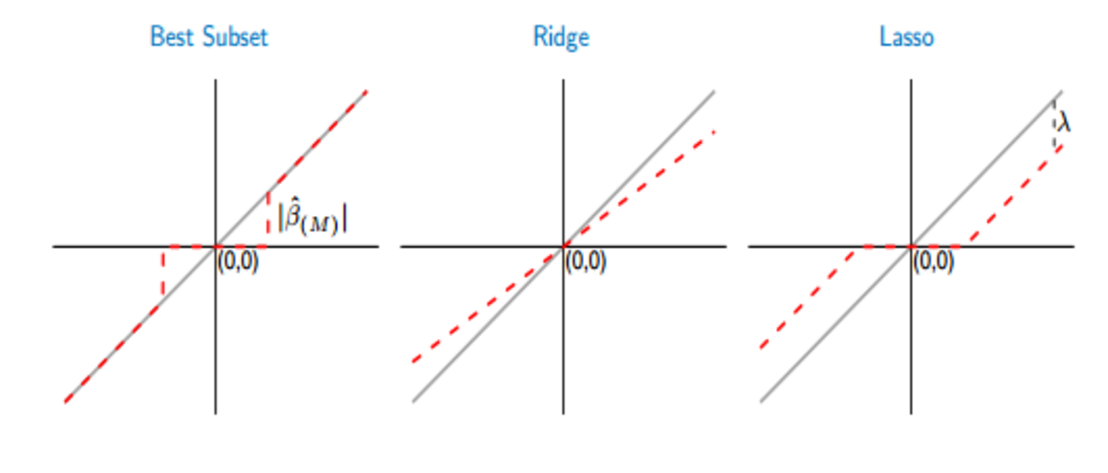
\includegraphics[width=0.8\textwidth]{lasso.pdf}
\caption{Estimated coefficients at coordinate descent in Lasso }
\label{fig:hist2}
\end{figure} 

 \subsection{\small{Least absolute shrinkage and selection operator}}
 Firstly we consider simple least absolute shrinkage and selection operator which is more preferable comparing to ridge, because instead of just shrinking coefficients in ridge regression, we reduce the dimension of $\Delta\phi$, selecting best-working features. 
 We consider the problem as 
 
$$\min_{\Delta \phi} \; (\Delta \phi, J^{\top}MJ \Delta \phi)-2(\Delta \phi, J^{\top}M\Delta r)$$
$$s.t. \sum\limits_{j=1}^{p} |\Delta\phi_j| \leqslant  s$$
That allows us use the quadratic programming approach of solving our optimization problem. For transformation constraints from  $\sum\limits_{j=1}^{p} |\Delta\phi_j| \leqslant s$ to $A\Delta\phi\leqslant s$ we do the following substitution $$\Delta\phi_i = \Delta\phi_i^+ - \Delta\phi_i^-, \; \text{where}  \;\Delta\phi_i^{+,-} \geqslant 0 \;\text{and}\; \Delta\phi_i^+ - \Delta\phi_i^- \geqslant 0 \;\;\forall i \in 1\dots p$$
Also, we denote by $Q=J^{\top}MJ$ and $c = -J^{\top}M\Delta r$, so there is a new formulation which could be transformed to the problem of quadratic programming with dimension of $2p$

$$ \min_{\Delta \phi^+,\; \Delta \phi^-} \; \frac{1}{2}(\Delta\phi_i^+ - \Delta\phi_i^-)^{\top}Q(\Delta\phi_i^+ - \Delta\phi_i^-) + c^{\top}(\Delta\phi_i^+ - \Delta\phi_i^-)$$
$$ s.t. \;\Delta \phi^+ + \Delta \phi^- \leqslant s$$
$$\Delta \phi^{+,-}\geqslant 0$$

It can be  rewritten in the matrix form as: 
\begin{gather}
\min_{\Delta \phi^+,\; \Delta \phi^-} \; \frac{1}{2}\begin{bmatrix} \Delta\phi_i^+ & \Delta\phi_i^- \end{bmatrix} \begin{bmatrix} Q & -Q \\ -Q 
& Q\end{bmatrix}\begin{bmatrix} \Delta\phi_i^+ \\ \Delta\phi_i^- \end{bmatrix}+\begin{bmatrix} c^{\top} & -c^{\top}\end{bmatrix}\begin{bmatrix} \Delta\phi_i^+ \\ \Delta\phi_i^- \end{bmatrix}
\end{gather}

\begin{gather}
\begin{bmatrix} I_{p}& I_{p} \\ -I_{2p} &\end{bmatrix}\begin{bmatrix} \Delta\phi_i^+ \\ \Delta\phi_i^- \end{bmatrix}\leq \begin{bmatrix} s_{p} \\ 0_{2p} \end{bmatrix}
\end{gather}

Where $I_{p}$ is the p-dimensional unit matrix, $s_{p}$ - p-dimensional vector, consisting only of the value s, and $0_{2p}$ is a $2p$-dimensional zero vector

 \subsection{\small{Elastic net regularization}}
Further, we analyze elastic-net regression in the application to finding conformational changes.  Lets consider the next formulation with  $\alpha > 0$ and discuss disadvantages

$$\min_{\Delta \phi} \; (\Delta \phi, J^{\top}MJ \Delta \phi)-2(\Delta \phi, J^{\top}M\Delta r) + \alpha(\Delta \phi, \Delta \phi) + (1-\alpha)\sum\limits_{j=1}^{p} |\Delta\phi_j|$$
The elastic net model is able to select groups of variables when they are highly correlated. It doesn't have the problem of selecting more than n predictors when $p \gg n$, but LASSO saturates in this situation. When there are highly correlated predictors, the LASSO tends to just pick one predictor out of the group. These disadvantages of LASSO could be overcome by the elastic net. But in our problem, it is not necessary, because we have $p \ll n$ and the real disadvantage is the computational cost. That will be due to the inevitable cross-validation of the relative weight of $L_1$ vs.$L_2$ penalty, $\alpha$, and that increases the computational cost by the number of values in the $\alpha$ grid. Another drawback, which can be also an advantage, is the flexibility of the estimator. Increased probability of overfitting comes with greater flexibility. It may be that the optimal $\alpha$ for the population and for the given sample size is 0, turning the elastic net into the lasso, but it possible to choose a different value due to chance\cite{RePEc:bla:jorssb:v:67:y:2005:i:5:p:768-768}. 


 \subsection{\small{Least angle regression }}
In addition, we review least angle regression as it produces a full piecewise linear solution path, which is simplifies cross-validation. The fact is that in the following there will be discussed the choice of the regularization parameter for our first model. Despite of this point the method has considerable disadvantages. With any amount of noise in the dependent variable and with high-dimensional multicollinear independent variables, there is no reason to believe that the selected variables will have a high probability of being the actual underlying causal variables. However, since LARS relies on an iterative update of residuals, it appears to be particularly sensitive to the effects of noise\cite{efron2004least}.  Furthermore, it is in our case that we have a lot of this, so we do not use LARS as the main strategy and as the solution of finding regularization parameter. 

 \section{Method}
 We use this formulation of Lasso from the  scikit-learn v0.20.1 library.
 The method that showed best results and most adequate answer is about coordinate decent. The formulation as usual like Lasso. We use coordinate descent. 
 $$\frac{1}{2n}\|\Delta r-J\Delta\phi\|_2^2+\alpha \|\Delta\phi\|_1$$

We split our dataset into 10 parts (10-fold cross validation)
We also used grid search automatically tuning hyperparameters on a parameter grid to choose the parameters with maximum  cross-validation score. We set initially grid with $\alpha\in[10^{-5}, 10^{-3}]$ with 30 values.   It works considerably slower then just Lasso using cross validation.



  
  \section{Implementation}
  
We use LassoCV and GreedSearchCV models for predicting $\Delta r$. $\Delta r$ is our target. 
 We take 30 pairs of initial dataset and for each pair calculate RMSD (initial, final) (it is given in existed code)  and RMSD(initial, predicted). Then we plot it on the one table to see correlation between two RMSD. The lower RMSD of prediced conformation and final conformation the more accurate the prediction so there should be strong correlation between this RMSD and the RMSD between the initial and final conformation. The larger the conformation change, the worse the reconstructed conformation. We tried to catch the pattern of correlation plotting results in two dimensional space ($RMSD_1$, $RMSD_2$) and checking their location relatively bisectrix. Also we estimated correlation of RMSD using linear approximation of data. We compared results of Lasso with cross validation, Lasso with grid-search cross-validation, Elastic net with cross-validation and Ridge regression.
 

\section{Results}

Finally, we analyze the properties of the torsional conformational changes obtained with Lasso based on grid-search and cross-validation showed reasonable results. 
We summarize the average RMSD between the reconstructed conformations and the target conformations for the six methods and showed, that least absolute shrinkage and selection operator model with cross-validation can work as good as  Ridge regression. 
\begin{center}

\begin{table}[h]
\begin{tabular}{|l|l|l|l|l|l|}
 \hline
LassoCV & EnCV & L=0  & Ridge M & Ridge С & LassoCVGS \\ \hline
2.39    & 2.17  & 6.79 & 1.71    & 1.53    & 1.74          \\ \hline
\end{tabular}
\end{table}
\end{center}
Two models: Grid search Lasso and Ridge regression type M yield accurate reconstructed structures, whose RMSD is on the average 1.7, i.e. the reconstructed conformations are approximately half the way between the initial and final conformational. As a result, sparse subset of collective coordinates in the torsion subspace can describe functional conformational changes in proteins.



\begin{figure}[h]
\centering
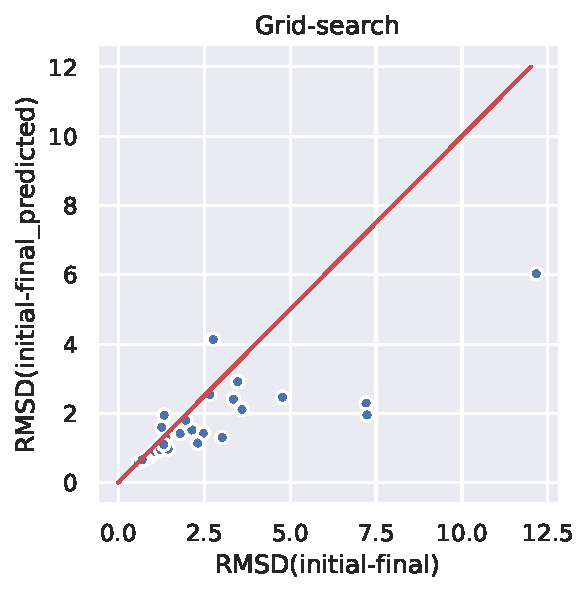
\includegraphics[width=0.5\textwidth]{Grid-search.pdf}
\caption{Correlation of RMSD in Grid search Lasso}
\label{fig:hist2}
\end{figure} 
\begin{figure}[h]
\centering
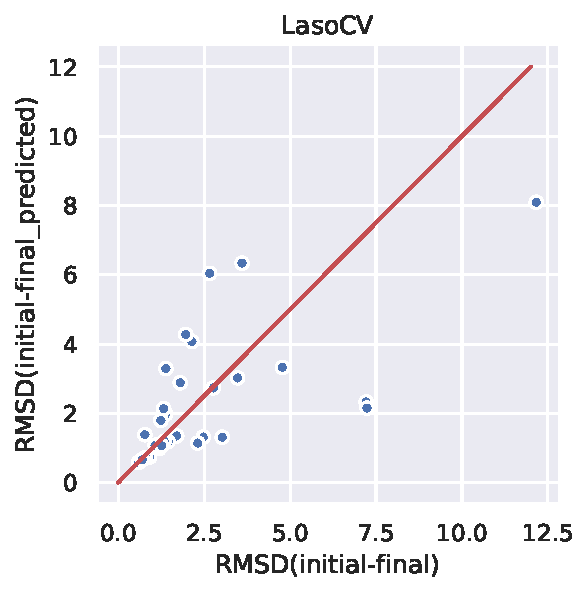
\includegraphics[width=0.5\textwidth]{LassoCV.pdf}
\caption{Correlation of RMSD in Lasso with cross validation}
\label{fig:hist2}
\end{figure} 
\begin{figure}[h]
\centering
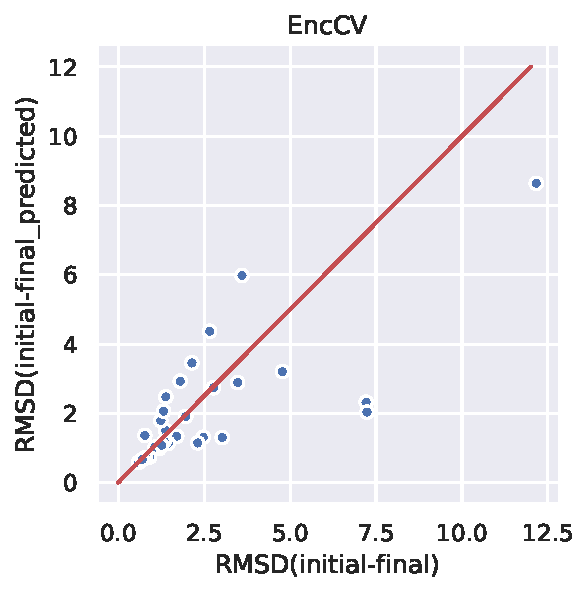
\includegraphics[width=0.5\textwidth]{EncCV.pdf}
\caption{Correlation of RMSD in Elasticnet with cross validation}
\label{fig:hist2}
\end{figure} 
\begin{figure}[h]
\centering
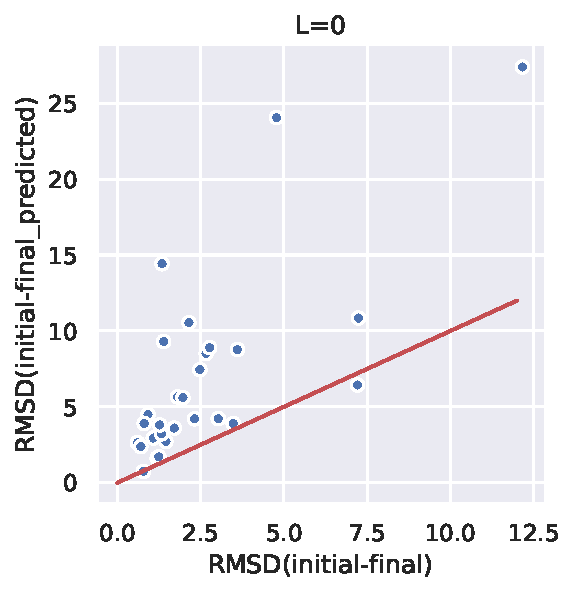
\includegraphics[width=0.5\textwidth]{L_0.pdf}
\caption{Correlation of RMSD in L=0 regression}
\label{fig:hist2}
\end{figure} 
\begin{figure}[h]
\centering
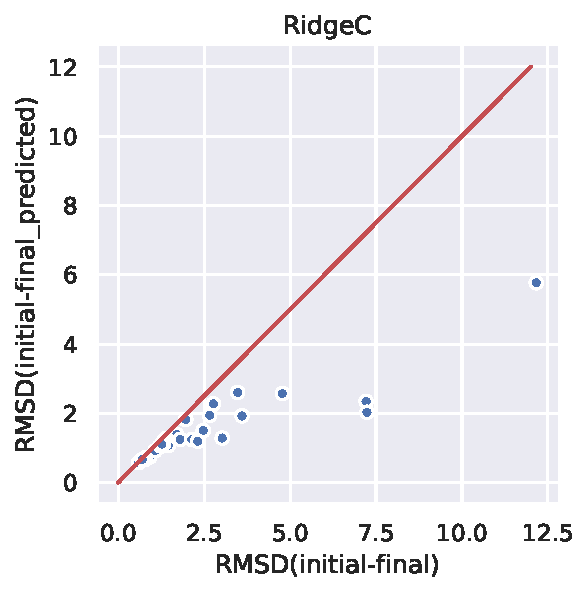
\includegraphics[width=0.5\textwidth]{RidgeC.pdf}
\caption{Correlation of RMSD in Ridge}
\label{fig:hist2}
\end{figure} 
\begin{figure}[h]
\centering
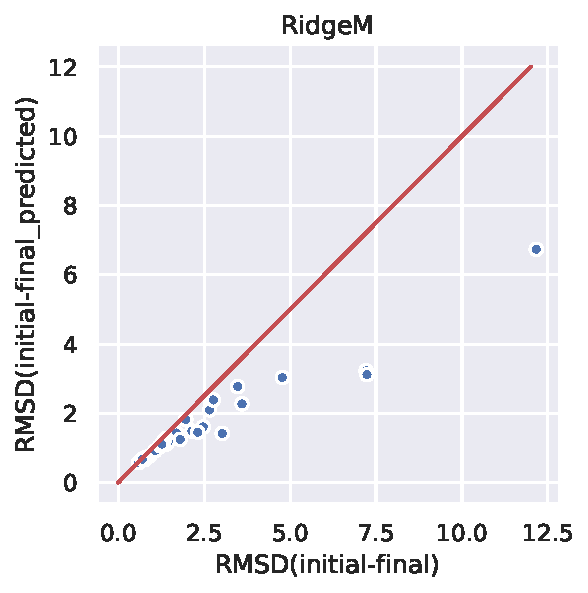
\includegraphics[width=0.5\textwidth]{RidgeM.pdf}
\caption{Correlation of RMSD in RidgeM}
\label{fig:hist2}
\end{figure} 

\begin{center}

\begin{figure}[h]
\centering
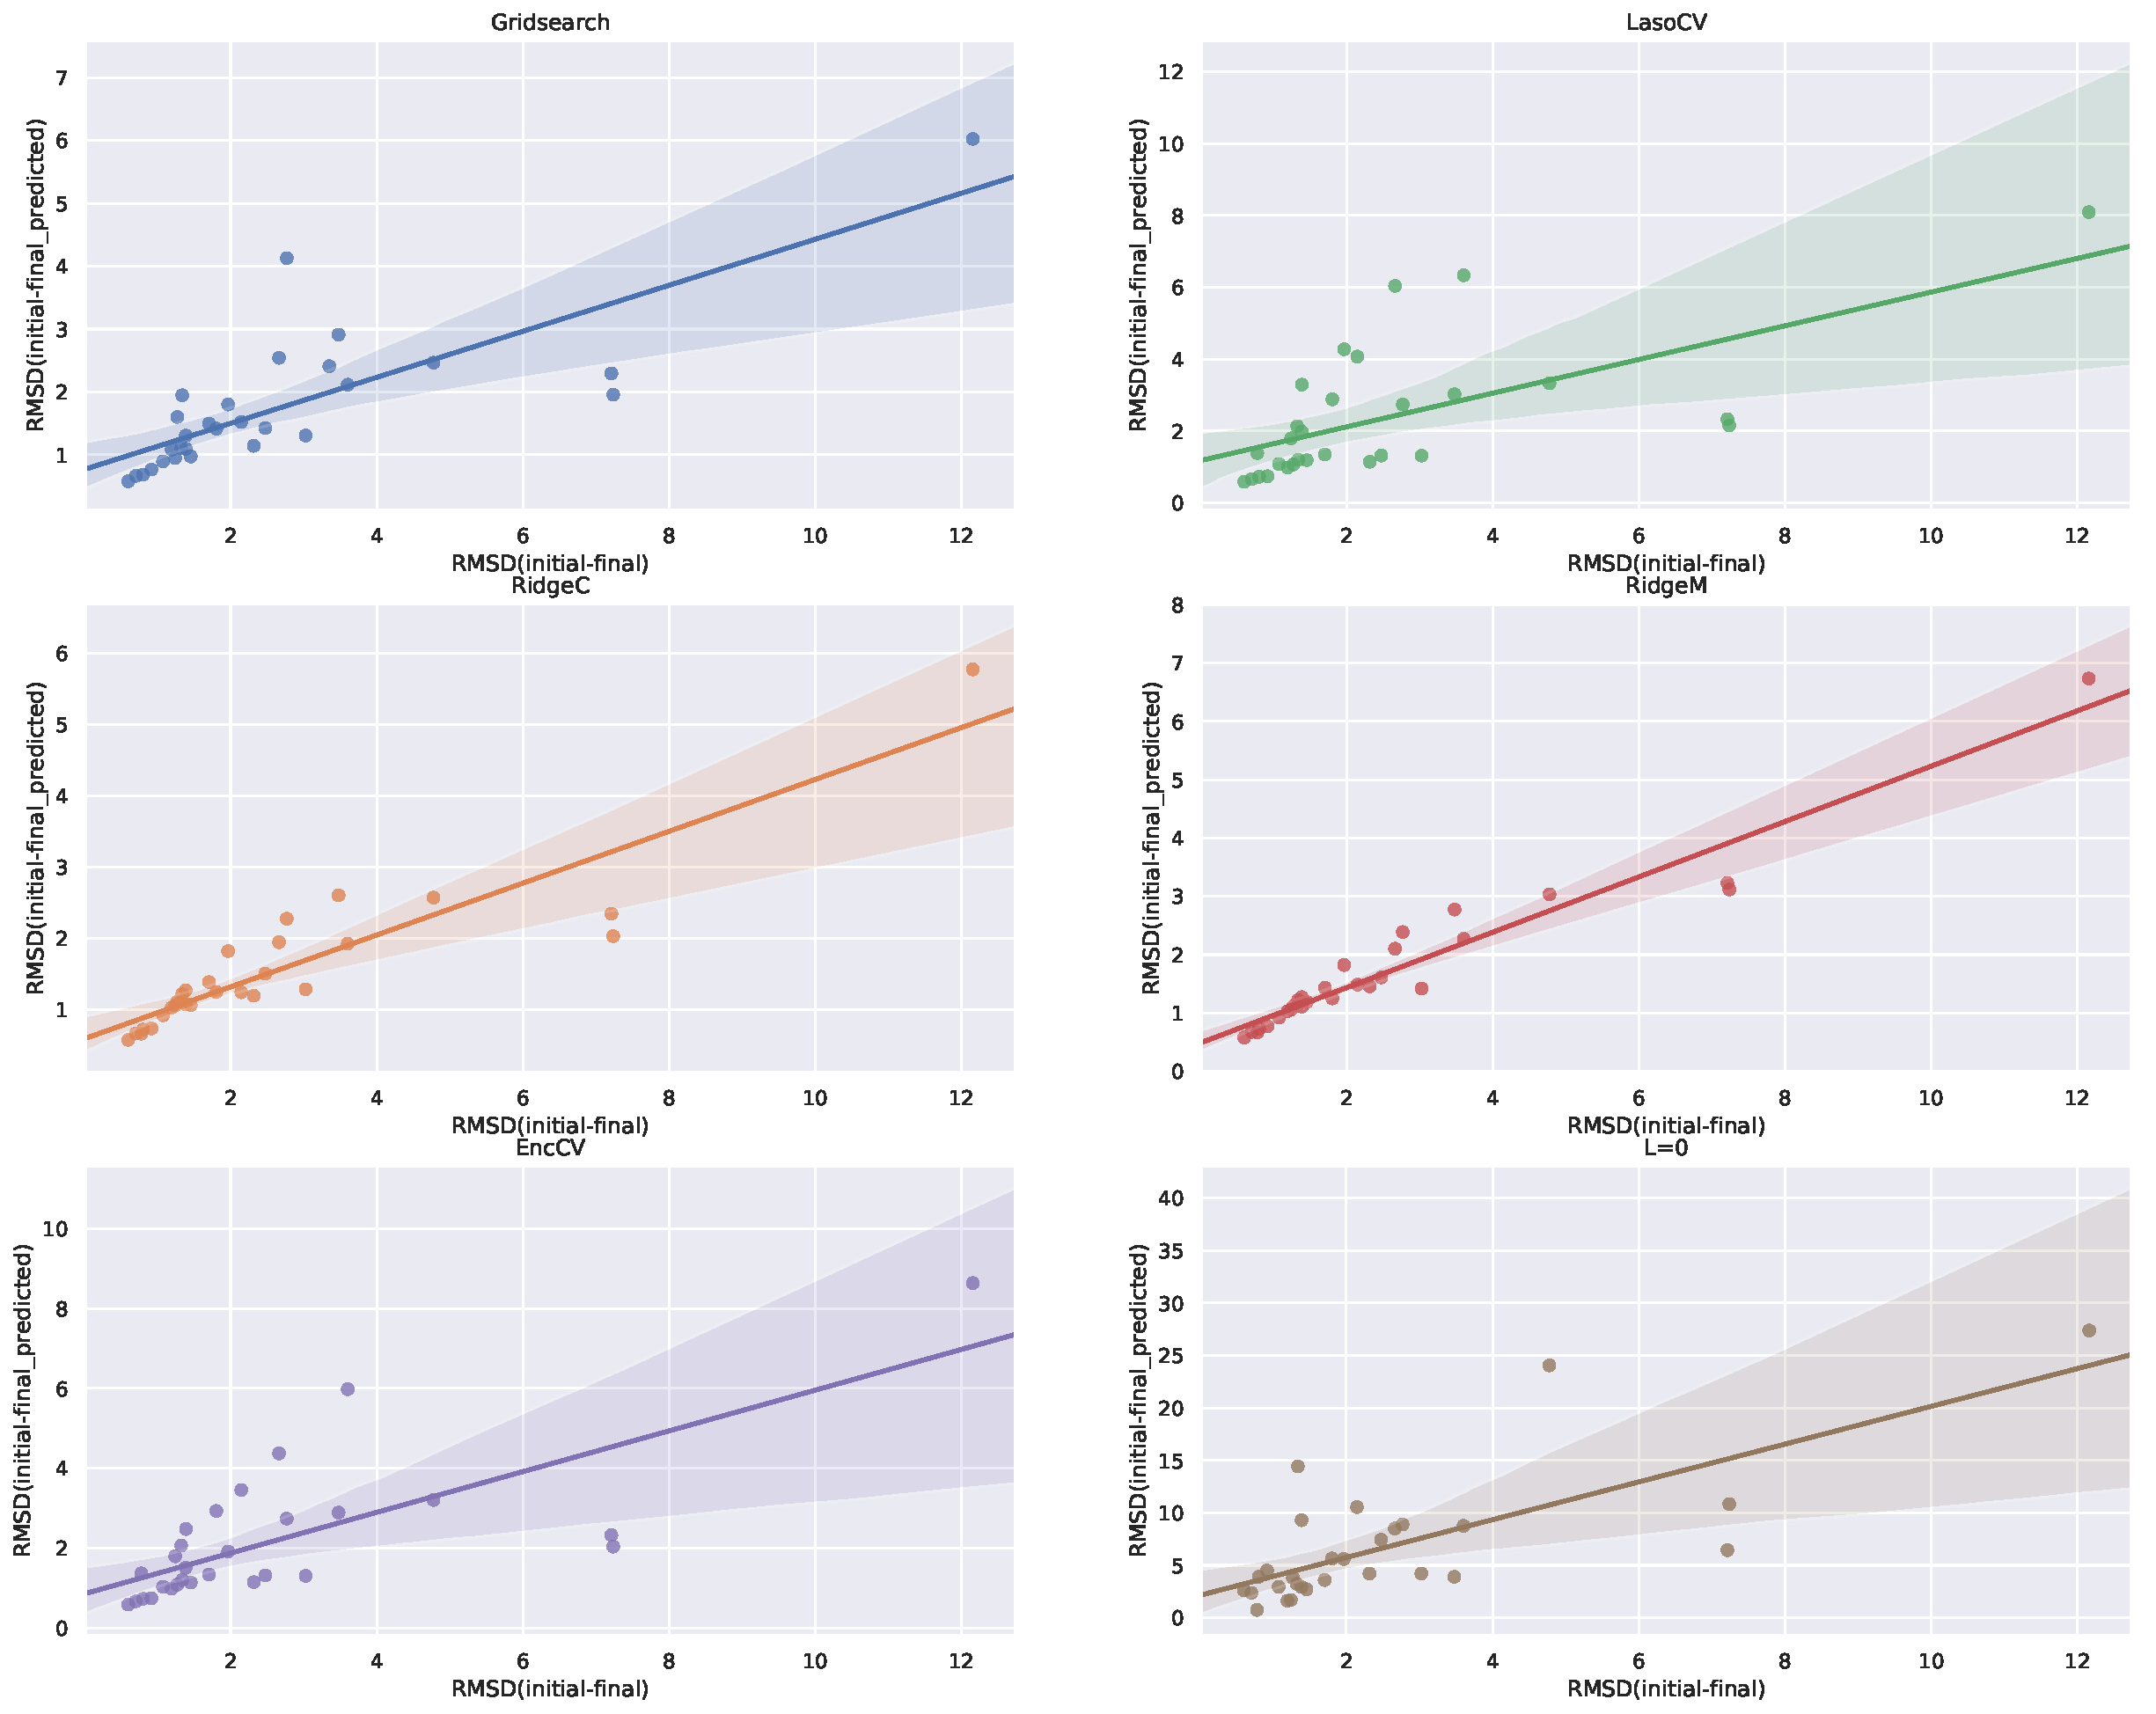
\includegraphics[width=1\textwidth]{Win.pdf}
\caption{Comparison of correlations of RMSD in all methods (using linear approximation). \\Root mean square deviation between the conformation modelled applying the torsional
differences on top of the initial conformation and the final conformation as a function of the RMSD between the
initial and the final conformation for six alternative methods for obtaining the torsional differences. }
\label{fig:hist2}
\end{figure} 

\end{center}
\clearpage
 \bibliographystyle{ieeetr}
 \bibliography{references}
        \end{document}
